\appendix
\setcounter{figure}{0}
\setcounter{table}{0}
\renewcommand{\theHfigure}{appendix.\arabic{figure}}
\renewcommand{\theHtable}{appendix.\arabic{table}}
\section{Extended evaluation and reproducibility}
\label{sec:appendix}
The appendix provides detailed outcomes, sensitivity cases and audits of the fixed experiment archive. Plotting scripts export the underlying observations as CSV and identify input logs by SHA-256 hashes. These calculations analyse existing runs without retraining controllers or replacing outcomes. Replication and single-seed cases are distinguished throughout.

\subsection{Detailed tabulations and development displays}
Tables and figures in this subsection give the development criteria, data partitions and numerical outcomes corresponding to the principal comparisons.
\begin{table}[htbp]
\centering\small
\caption{Development-set selection of FedGrid variants. Damage is in dollars over the validation weeks and uses a bill-plus-curtailment score. The post-hoc 4.0\% bound uses the rounded original rejection rate. Rejection pools differ: 21 original runs versus 15 per complete candidate. The last column is the mean of per-run maximum honest-household rejection, not the maximum across runs.}
\label{tab:selection_candidates}
\resizebox{\linewidth}{!}{%
\begin{tabular}{llll}
\toprule
Variant & Worst validation damage & Honest rejection (\%) & Mean run maximum (\%) \\
\midrule
original & 26.0 & 2.0 & 18.0 \\
filter\_first & 19.0 & 3.8 & 28.2 \\
filter\_first\_clip2 & 14.5 & 3.4 & 27.3 \\
filter\_first\_guard & 21.2 & 6.7 & 27.6 \\
filter\_first\_home\_trust & 6.2 & 30.8 & 70.6 \\
without\_clip & 15.3 & 3.5 & 29.4 \\
\bottomrule
\end{tabular}}
\end{table}


\begin{figure}[htbp]
\centering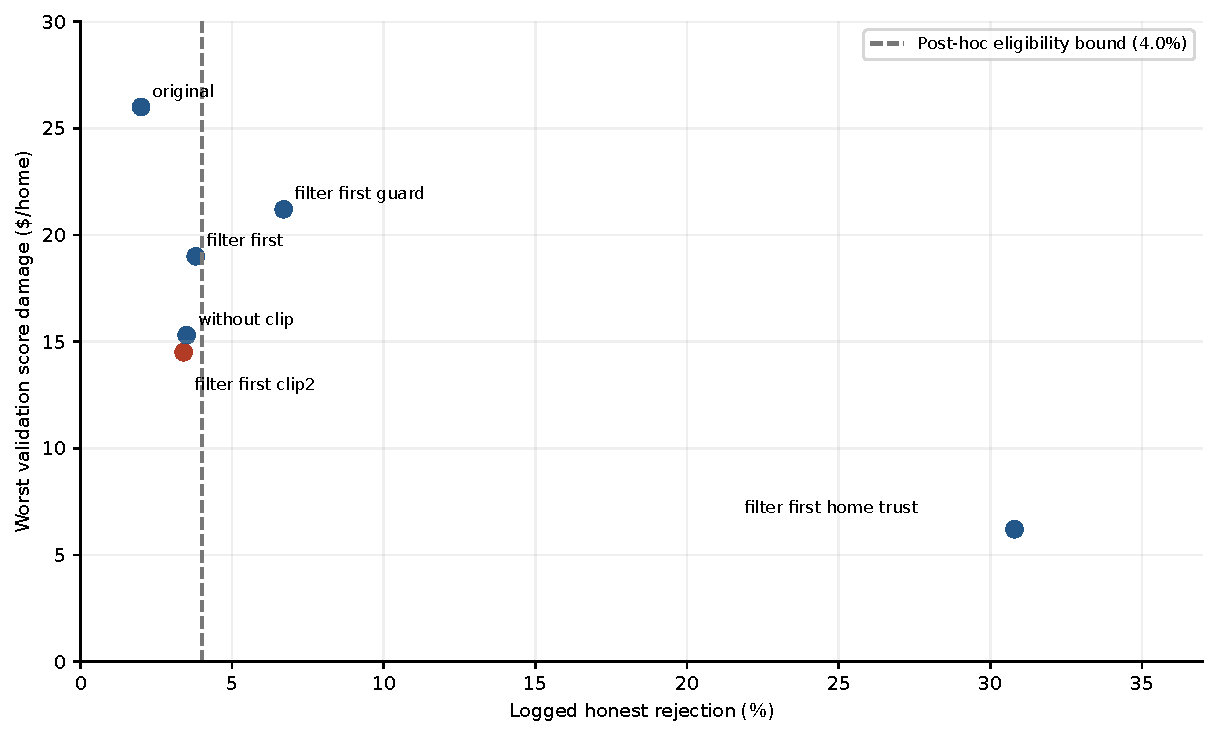
\includegraphics[width=.9\linewidth]{figures/selection_candidates.pdf}
\caption{Candidate selection on validation data, seeds 0--2. The dashed rejection bound was introduced after inspecting candidate results. Validation damage uses a bill-plus-curtailment score over validation weeks; it is not annual evaluation bill damage.}
\label{fig:selection}
\end{figure}

\begin{figure}[htbp]
\centering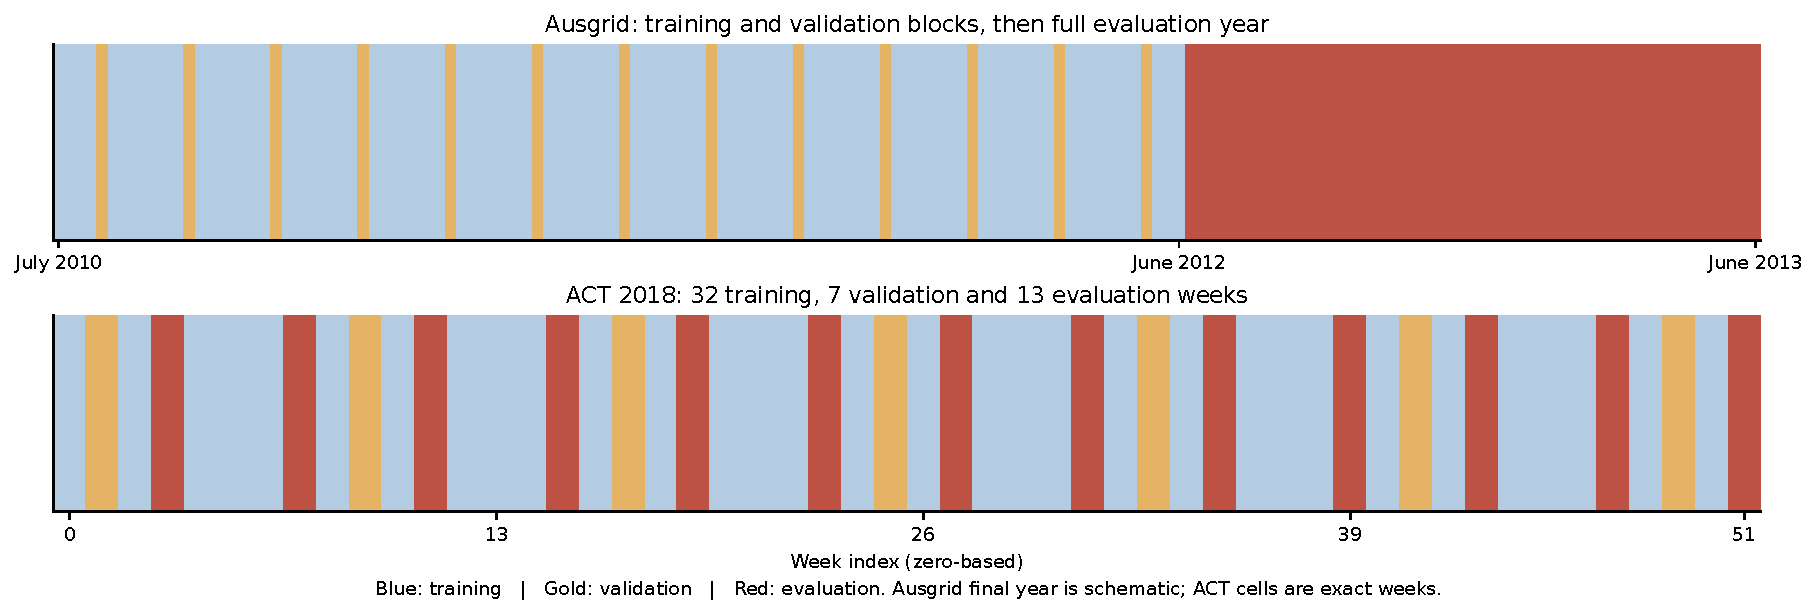
\includegraphics[width=\linewidth]{figures/data_splits.pdf}
\caption{Ausgrid and ACT partitions. The Ausgrid evaluation year is shown schematically after the 104 seven-day development blocks. ACT cells show the exact interleaved weekly assignment. New learning seeds do not create a new chronological holdout. Diagram code was assisted by OpenAI Codex (exact deployed model identifier unavailable).}
\label{fig:splits}
\end{figure}

\begin{table}[htbp]
\centering\small
\caption{Clean 500-day learning with validation-selected policies, Ausgrid. Mean $\pm$ 95\% interval half-width [seeds]; deterministic baselines have one observation. MSL charging is a street-wide total; bills and curtailment are household averages. Cycles are total throughput divided by twice total fleet capacity.}
\label{tab:clean_energy}
\resizebox{\linewidth}{!}{%
\begin{tabular}{lllll}
\toprule
Method & Bill (\$/yr) & Curtailment (kWh/yr) & Cycles/yr & MSL charge (kWh) \\
\midrule
Idle & 1457.8 [1] & 537.7 [1] & 0.0 [1] & 0.0 [1] \\
Rule & 953.0 [1] & 473.2 [1] & 77.5 [1] & 1971.1 [1] \\
Local SAC & 963.8 $\pm$ 61.2 [3] & 134.8 $\pm$ 49.4 [3] & 247.4 $\pm$ 39.4 [3] & 13307.6 $\pm$ 2085.6 [3] \\
FedAvg & 954.3 $\pm$ 79.0 [3] & 144.6 $\pm$ 89.9 [3] & 255.9 $\pm$ 48.6 [3] & 12735.2 $\pm$ 4074.3 [3] \\
FedProx & 947.3 $\pm$ 65.2 [3] & 153.5 $\pm$ 84.8 [3] & 252.7 $\pm$ 38.8 [3] & 12396.6 $\pm$ 3452.8 [3] \\
Central SAC & 879.1 $\pm$ 117.7 [3] & 137.9 $\pm$ 160.3 [3] & 277.7 $\pm$ 34.9 [3] & 13872.7 $\pm$ 4775.5 [3] \\
MPC oracle & 591.0 [1] & 62.9 [1] & 213.4 [1] & 14942.1 [1] \\
\bottomrule
\end{tabular}}
\end{table}


\begin{table}[htbp]
\centering\small
\caption{Annual bill damage on ACT. Mean $\pm$ 95\% interval half-width [seeds], dollars per household. Transfer coverage differs by method.}
\label{tab:act_damage}
\resizebox{\linewidth}{!}{%
\begin{tabular}{lllllll}
\toprule
Method & Flip & Scale & Noise & Normalized & Meter & Reward \\
\midrule
FedAvg & 123.1 $\pm$ 89.9 [3] & 23.5 $\pm$ 151.6 [3] & 758.9 $\pm$ 123.1 [3] & 757.7 $\pm$ 384.8 [3] & 21.7 $\pm$ 165.9 [3] & 131.4 $\pm$ 138.9 [3] \\
Median & 87.8 $\pm$ 169.2 [3] & -64.6 $\pm$ 47.8 [3] & 2.3 $\pm$ 177.8 [3] & 356.4 $\pm$ 450.4 [3] & 12.2 $\pm$ 63.5 [3] & 186.9 $\pm$ 14.1 [3] \\
Trimmed mean & 65.8 $\pm$ 194.7 [3] & -82.9 $\pm$ 81.4 [3] & 6.5 $\pm$ 149.5 [3] & 181.2 $\pm$ 67.6 [3] & 8.5 $\pm$ 109.7 [3] & 168.6 $\pm$ 70.4 [3] \\
Krum & 12.2 $\pm$ 284.5 [3] & -53.1 $\pm$ 288.0 [3] & -60.7 $\pm$ 161.9 [3] & -75.2 $\pm$ 10.1 [3] & -1.5 $\pm$ 179.7 [3] & -47.2 $\pm$ 130.2 [3] \\
FLTrust & 15.5 $\pm$ 148.9 [3] & -0.4 $\pm$ 4.8 [3] & 14.5 $\pm$ 224.9 [3] & 11.3 $\pm$ 134.3 [3] & -18.1 $\pm$ 152.3 [3] & 21.9 $\pm$ 147.8 [3] \\
FLAME & 55.9 $\pm$ 162.0 [3] & 38.9 $\pm$ 96.6 [3] & 13.8 $\pm$ 109.4 [3] & 59.7 $\pm$ 110.7 [3] & 38.2 $\pm$ 91.1 [3] & 32.6 $\pm$ 101.8 [3] \\
TAFDRL-style & 55.2 $\pm$ 106.0 [3] & 39.2 $\pm$ 36.1 [3] & 27.4 $\pm$ 101.1 [3] & 88.3 $\pm$ 132.4 [3] & 23.4 $\pm$ 62.3 [3] & 23.7 $\pm$ 25.3 [3] \\
TAFDRL-style tuned & 19.4 $\pm$ 61.8 [3] & 24.6 $\pm$ 59.1 [3] & 14.9 $\pm$ 111.1 [3] & 140.1 $\pm$ 209.9 [3] & 27.8 $\pm$ 106.1 [3] & 19.5 $\pm$ 86.0 [3] \\
FedGrid original & 73.6 $\pm$ 84.5 [3] & 3.9 $\pm$ 44.1 [3] & 35.2 $\pm$ 141.2 [3] & 165.6 $\pm$ 86.7 [3] & 35.4 $\pm$ 135.5 [3] & 117.8 $\pm$ 54.2 [3] \\
FedGrid final & 93.5 $\pm$ 55.2 [3] & 44.3 $\pm$ 40.1 [3] & 25.1 $\pm$ 81.1 [3] & 5.0 $\pm$ 16.0 [3] & 38.7 $\pm$ 101.2 [3] & 112.0 $\pm$ 77.3 [3] \\
\bottomrule
\end{tabular}}
\end{table}


\begin{table}[htbp]
\centering\small
\caption{Paired change in attack damage, final minus original FedGrid, in dollars per household annually. Negative values favour the revision. Intervals are descriptive, unadjusted Student-t intervals; transfer uses only matched seeds 3--4.}
\label{tab:paired_revision}
\resizebox{\linewidth}{!}{%
\begin{tabular}{llll}
\toprule
Attack & Ausgrid [5] & ACT [3] & Transfer [2] \\
\midrule
Flip & -10.4 $\pm$ 23.5 [5] & 20.0 $\pm$ 34.1 [3] & -22.8 $\pm$ 229.8 [2] \\
Scale & -5.3 $\pm$ 16.0 [5] & 40.4 $\pm$ 80.3 [3] & -1.6 $\pm$ 135.7 [2] \\
Noise & -28.4 $\pm$ 20.1 [5] & -10.1 $\pm$ 62.8 [3] & -34.6 $\pm$ 132.0 [2] \\
Normalized & -76.8 $\pm$ 67.5 [5] & -160.6 $\pm$ 97.5 [3] & -74.1 $\pm$ 175.9 [2] \\
Meter & 13.6 $\pm$ 38.2 [5] & 3.3 $\pm$ 42.4 [3] & -16.2 $\pm$ 430.4 [2] \\
Reward & 14.6 $\pm$ 32.2 [5] & -5.8 $\pm$ 58.6 [3] & 11.7 $\pm$ 431.6 [2] \\
\bottomrule
\end{tabular}}
\end{table}


\begin{table}[htbp]
\centering\small
\caption{Logged honest update rejection on Ausgrid, nominal 30\% compromise, seeds 0--4 where available. Entries are mean $\pm$ 95\% interval half-width [observed seeds]. Admission semantics differ across defences.}
\label{tab:rejection}
\resizebox{\linewidth}{!}{%
\begin{tabular}{llllllll}
\toprule
Method & None & Flip & Scale & Noise & Normalized & Meter & Reward \\
\midrule
Krum & 97.2 $\pm$ 0.0 [4] & 96.0 $\pm$ 0.0 [4] & 96.0 $\pm$ 0.0 [4] & 96.0 $\pm$ 0.0 [4] & 96.4 $\pm$ 0.1 [4] & 96.0 $\pm$ 0.0 [5] & 96.0 $\pm$ 0.1 [5] \\
FLTrust & 31.6 $\pm$ 4.8 [5] & 28.4 $\pm$ 4.2 [5] & 31.7 $\pm$ 8.3 [5] & 28.3 $\pm$ 2.8 [5] & 16.2 $\pm$ 4.0 [5] & 29.0 $\pm$ 3.8 [5] & 27.9 $\pm$ 5.5 [5] \\
FLAME & 47.0 $\pm$ 0.2 [5] & 34.9 $\pm$ 2.9 [5] & 23.9 $\pm$ 0.1 [5] & 23.9 $\pm$ 0.1 [5] & 46.3 $\pm$ 2.1 [5] & 24.2 $\pm$ 0.2 [5] & 24.3 $\pm$ 0.2 [5] \\
TAFDRL-style & 8.5 $\pm$ 0.8 [5] & 3.1 $\pm$ 1.2 [5] & 0.1 $\pm$ 0.1 [5] & 0.1 $\pm$ 0.0 [5] & 31.1 $\pm$ 3.7 [5] & 1.5 $\pm$ 0.6 [5] & 2.9 $\pm$ 1.1 [5] \\
TAFDRL-style tuned & 20.4 $\pm$ 2.2 [5] & 11.3 $\pm$ 1.8 [5] & 0.2 $\pm$ 0.2 [5] & 0.1 $\pm$ 0.0 [5] & 53.0 $\pm$ 7.7 [5] & 3.1 $\pm$ 1.3 [5] & 7.1 $\pm$ 3.2 [5] \\
FedGrid original & 3.2 $\pm$ 0.7 [5] & 0.4 $\pm$ 0.5 [5] & 2.3 $\pm$ 0.9 [5] & 0.2 $\pm$ 0.3 [5] & 4.6 $\pm$ 1.8 [5] & 1.1 $\pm$ 0.5 [5] & 2.5 $\pm$ 1.5 [5] \\
FedGrid final & 6.2 $\pm$ 1.3 [5] & 2.1 $\pm$ 0.7 [5] & 0.8 $\pm$ 0.6 [5] & 0.6 $\pm$ 0.3 [5] & 6.5 $\pm$ 3.8 [5] & 3.4 $\pm$ 0.8 [5] & 4.5 $\pm$ 1.4 [5] \\
\bottomrule
\end{tabular}}
\end{table}


\begin{table}[htbp]
\centering\small
\caption{Electrical outcomes for no-attack last-policy runs. Means and 95\% interval half-widths [observed seeds] of evaluation-run metrics. A run-level voltage maximum or transformer peak is computed before averaging; these are not pooled worst-case bounds.}
\label{tab:electrical}
\resizebox{\linewidth}{!}{%
\begin{tabular}{lllll}
\toprule
Setting & Method & Over 253 V (\%) & Run maximum (V) & Transformer peak (\%) \\
\midrule
Ausgrid & FedAvg & 0.0 $\pm$ 0.0 [5] & 251.2 $\pm$ 1.6 [5] & 66.0 $\pm$ 9.0 [4] \\
Ausgrid & FLTrust & 0.0 $\pm$ 0.0 [5] & 251.1 $\pm$ 1.1 [5] & 63.8 $\pm$ 5.1 [5] \\
Ausgrid & FLAME & 0.0 $\pm$ 0.0 [5] & 251.3 $\pm$ 0.7 [5] & 64.6 $\pm$ 2.5 [5] \\
Ausgrid & TAFDRL-style tuned & 0.0 $\pm$ 0.0 [5] & 251.4 $\pm$ 1.2 [5] & 66.4 $\pm$ 5.8 [5] \\
Ausgrid & FedGrid original & 0.0 $\pm$ 0.0 [5] & 251.9 $\pm$ 1.6 [5] & 66.1 $\pm$ 7.3 [5] \\
Ausgrid & FedGrid final & 0.0 $\pm$ 0.0 [5] & 252.1 $\pm$ 1.5 [5] & 66.8 $\pm$ 5.8 [5] \\
ACT & FedAvg & 0.0 $\pm$ 0.0 [3] & 250.2 $\pm$ 1.4 [3] & 70.1 $\pm$ 18.0 [3] \\
ACT & FLTrust & 0.0 $\pm$ 0.0 [3] & 250.2 $\pm$ 1.6 [3] & 63.6 $\pm$ 28.4 [3] \\
ACT & FLAME & 0.0 $\pm$ 0.0 [3] & 250.0 $\pm$ 0.7 [3] & 63.4 $\pm$ 18.7 [3] \\
ACT & TAFDRL-style tuned & 0.0 $\pm$ 0.0 [3] & 250.4 $\pm$ 4.1 [3] & 67.3 $\pm$ 31.1 [3] \\
ACT & FedGrid original & 0.0 $\pm$ 0.0 [3] & 250.6 $\pm$ 1.7 [3] & 67.4 $\pm$ 22.2 [3] \\
ACT & FedGrid final & 0.0 $\pm$ 0.0 [3] & 250.1 $\pm$ 1.0 [3] & 66.3 $\pm$ 22.5 [3] \\
\bottomrule
\end{tabular}}
\end{table}


\begin{figure}[htbp]
\centering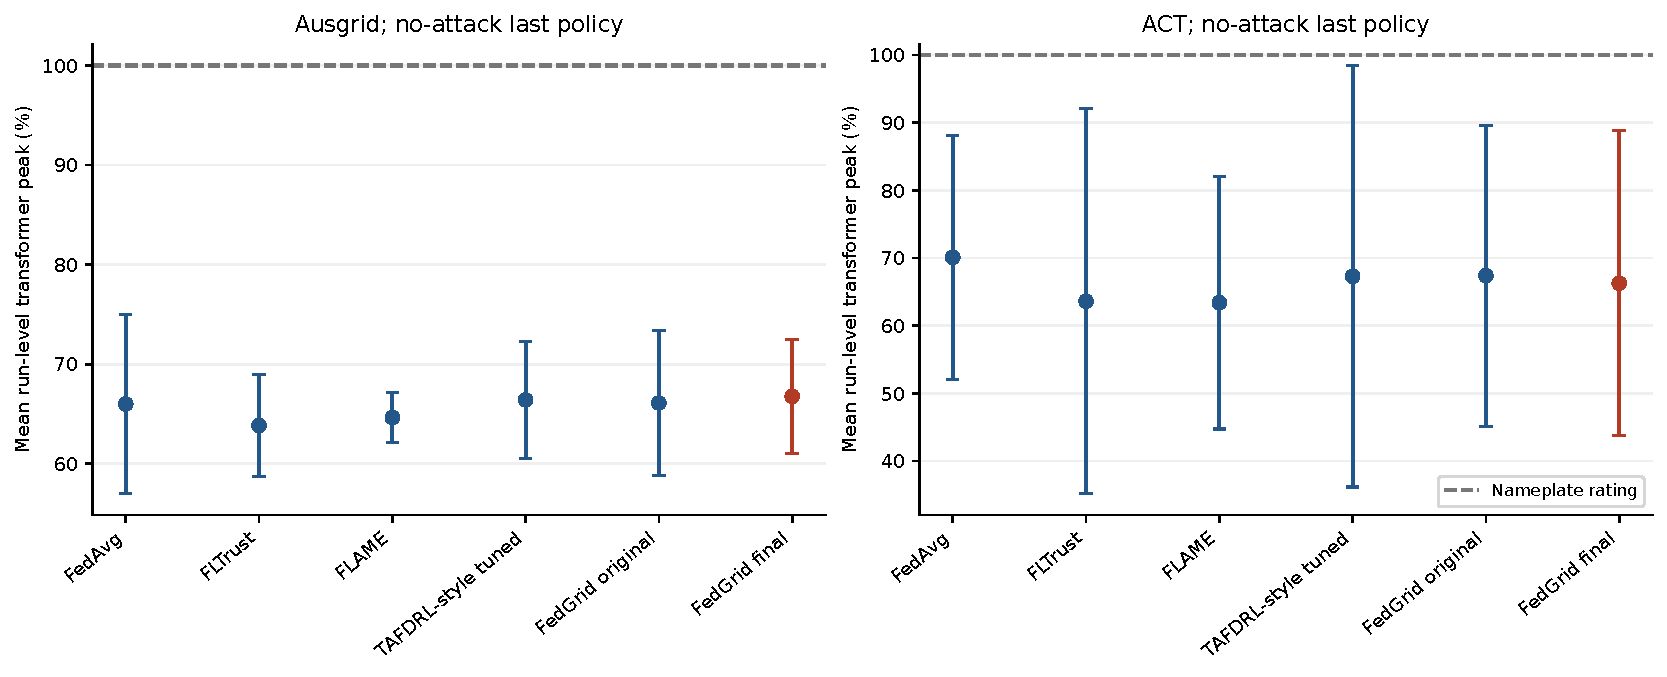
\includegraphics[width=\linewidth]{figures/electrical.pdf}
\caption{Run-level peak transformer loading in no-attack last-policy references, with seed means and 95\% interval half-widths. Ausgrid uses five seeds and ACT three, except the legacy FedAvg transformer statistic has four Ausgrid observations. The dashed line marks nameplate loading; it is not an enforced simulator constraint.}
\label{fig:electrical}
\end{figure}

\subsection{Transfer outcomes with explicit coverage}
Table~\ref{tab:transfer_damage} reports transfer outcomes using five seeds for the final variants and seeds 3--4 for the other configurations. Revision effects use the common-seed differences in Table~\ref{tab:paired_revision}, rather than differences between these unequal aggregate means.
\begin{table}[htbp]
\centering\small
\caption{Annual bill damage on ACT transfer. Mean $\pm$ 95\% interval half-width [seeds], dollars per household. Transfer coverage differs by method.}
\label{tab:transfer_damage}
\resizebox{\linewidth}{!}{%
\begin{tabular}{lllllll}
\toprule
Method & Flip & Scale & Noise & Normalized & Meter & Reward \\
\midrule
FedAvg & 143.6 $\pm$ 317.5 [2] & 87.5 $\pm$ 1060.1 [2] & 756.3 $\pm$ 920.3 [2] & 842.0 $\pm$ 1124.3 [2] & 9.0 $\pm$ 277.0 [2] & 106.7 $\pm$ 566.9 [2] \\
Median & 110.1 $\pm$ 692.9 [2] & -14.1 $\pm$ 377.8 [2] & -3.5 $\pm$ 255.1 [2] & 190.6 $\pm$ 914.7 [2] & -11.7 $\pm$ 74.6 [2] & 131.9 $\pm$ 217.3 [2] \\
Trimmed mean & 86.4 $\pm$ 47.0 [2] & -20.6 $\pm$ 269.5 [2] & -0.2 $\pm$ 242.8 [2] & 369.2 $\pm$ 136.8 [2] & 16.6 $\pm$ 55.8 [2] & 141.9 $\pm$ 214.2 [2] \\
Krum & -22.8 $\pm$ 1103.8 [2] & -5.5 $\pm$ 827.7 [2] & 49.2 $\pm$ 21.4 [2] & 61.4 $\pm$ 525.0 [2] & -7.6 $\pm$ 816.2 [2] & 20.7 $\pm$ 1027.3 [2] \\
FLTrust & -4.2 $\pm$ 81.5 [2] & 4.3 $\pm$ 70.4 [2] & -35.4 $\pm$ 32.9 [2] & 83.5 $\pm$ 456.3 [2] & 30.0 $\pm$ 15.4 [2] & 61.3 $\pm$ 85.0 [2] \\
FLAME & 66.2 $\pm$ 266.8 [2] & 4.6 $\pm$ 134.9 [2] & 8.0 $\pm$ 371.7 [2] & 26.6 $\pm$ 47.8 [2] & 12.3 $\pm$ 379.3 [2] & -8.3 $\pm$ 52.2 [2] \\
TAFDRL-style & 108.7 $\pm$ 17.6 [2] & 5.8 $\pm$ 207.5 [2] & -4.9 $\pm$ 293.8 [2] & 105.9 $\pm$ 499.9 [2] & 16.3 $\pm$ 35.4 [2] & 7.0 $\pm$ 238.2 [2] \\
TAFDRL-style tuned & 49.9 $\pm$ 29.6 [5] & 28.8 $\pm$ 32.8 [5] & 4.0 $\pm$ 15.7 [5] & 35.8 $\pm$ 98.4 [5] & 17.2 $\pm$ 21.3 [5] & 24.4 $\pm$ 44.9 [5] \\
FedGrid original & 121.6 $\pm$ 310.5 [2] & 0.3 $\pm$ 61.2 [2] & 75.2 $\pm$ 1.8 [2] & 113.5 $\pm$ 42.2 [2] & 29.1 $\pm$ 279.9 [2] & 110.1 $\pm$ 588.4 [2] \\
FedGrid final & 78.9 $\pm$ 47.0 [5] & -12.0 $\pm$ 19.4 [5] & 21.4 $\pm$ 29.1 [5] & -3.3 $\pm$ 60.0 [5] & 28.3 $\pm$ 23.4 [5] & 103.9 $\pm$ 39.6 [5] \\
\bottomrule
\end{tabular}}
\end{table}


\subsection{Compromised share}
Normalized-attack sensitivity uses seed 0 at nominal compromised shares of 10, 20, 30 and 40\%. Trimmed mean and Krum change their assumed faulty count and use share-matched no-attack references; other methods use their seed-0 30\% reference. Final FedGrid has lower observed damage than FedAvg in these cases. Four settings from one seed do not, however, identify a resilience threshold, particularly when a capacity band may contain a compromised majority.
\begin{table}[htbp]
\centering\small
\caption{Normalized-attack annual bill damage by nominal compromised share, seed 0 only. Trimmed mean and Krum use share-matched references; other methods use their 30\% no-attack reference.}
\label{tab:attack_share}
\resizebox{\linewidth}{!}{%
\begin{tabular}{lllll}
\toprule
Method & 10\% & 20\% & 30\% & 40\% \\
\midrule
FedAvg & 297.7 [1] & 446.5 [1] & 516.1 [1] & 516.2 [1] \\
Median & 50.4 [1] & 94.0 [1] & 267.9 [1] & 301.3 [1] \\
Trimmed mean & 48.7 [1] & 147.2 [1] & 192.5 [1] & 394.9 [1] \\
Krum & 75.6 [1] & 76.9 [1] & -37.5 [1] & 110.9 [1] \\
FLTrust & -42.8 [1] & -41.4 [1] & -32.9 [1] & -7.9 [1] \\
FLAME & -21.3 [1] & 31.7 [1] & -25.5 [1] & 39.1 [1] \\
TAFDRL-style & 25.1 [1] & 37.8 [1] & 12.6 [1] & 121.8 [1] \\
TAFDRL-style tuned & -6.4 [1] & -9.9 [1] & -35.0 [1] & 13.5 [1] \\
FedGrid original & 23.9 [1] & 79.8 [1] & 94.8 [1] & 105.9 [1] \\
FedGrid final & 16.6 [1] & 18.7 [1] & -19.4 [1] & 17.9 [1] \\
\bottomrule
\end{tabular}}
\end{table}

\begin{figure}[htbp]
\centering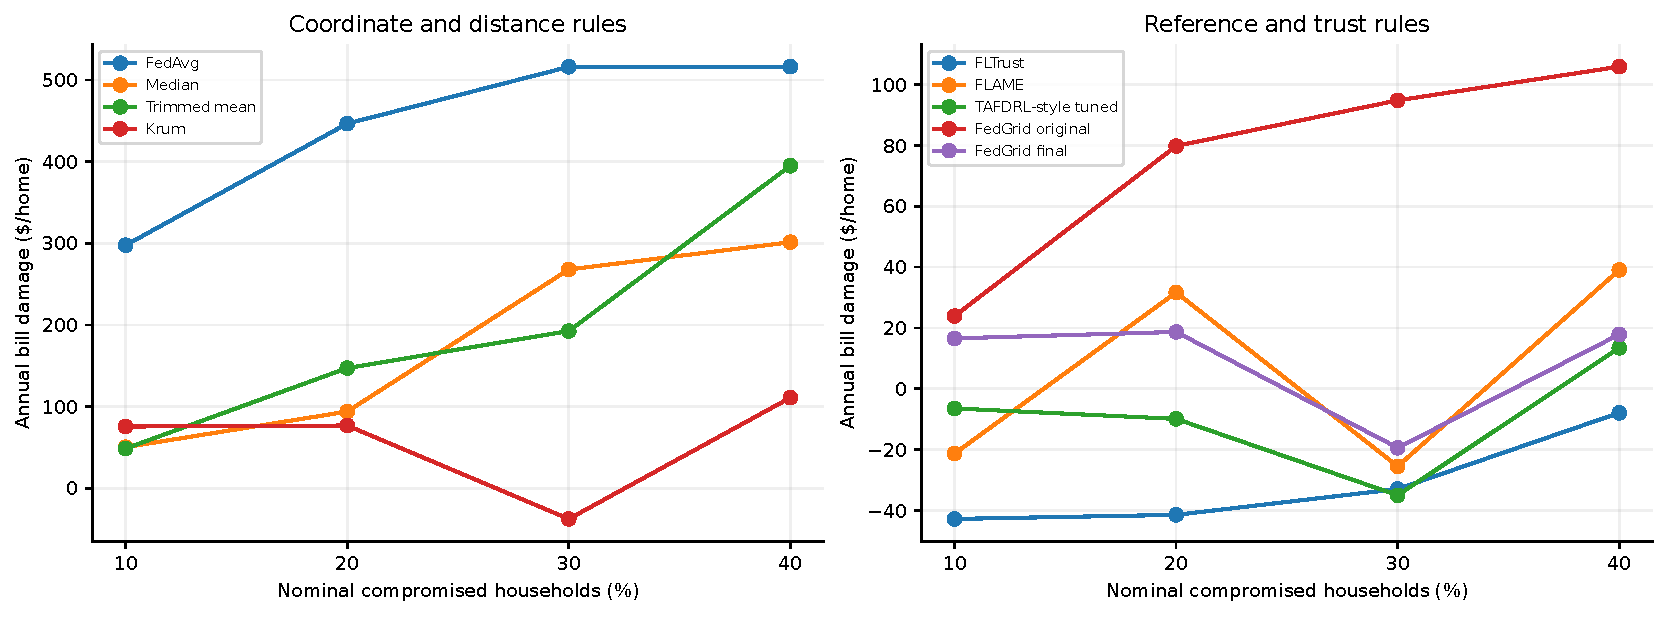
\includegraphics[width=\linewidth]{figures/attack_share.pdf}
\caption{Normalized-attack damage versus nominal compromised share, seed 0 only. Separate panels improve readability; vertical scales differ. Each point is a single experimental difference with no seed uncertainty interval.}
\label{fig:shares}
\end{figure}

\subsection{Ablation and operation order}
Each original-method ablation removes clipping, grouping or trust separately. Without clipping, Normalized damage is lower in these three seeds; removing grouping or trust does not reproduce the final configuration's outcome. The final configuration jointly changes filter order and clipping bound. These comparisons indicate an interaction worth examining, but do not isolate the cause of the combined revision's improvement.
\begin{table}[htbp]
\centering\small
\caption{Normalized-attack damage and logged honest rejection for the original FedGrid ablations and final variant, seeds 0--2. The final variant changes both filter order and clipping multiplier; it is not a one-factor ablation.}
\label{tab:ablation}
\resizebox{\linewidth}{!}{%
\begin{tabular}{lll}
\toprule
Variant & Damage (\$/home/yr) & Honest rejection (\%) \\
\midrule
original & 89.9 $\pm$ 25.7 [3] & 4.9 $\pm$ 2.9 [3] \\
without\_clip & -0.3 $\pm$ 102.8 [3] & 6.8 $\pm$ 3.0 [3] \\
without\_groups & 125.0 $\pm$ 90.5 [3] & 3.2 $\pm$ 3.1 [3] \\
without\_trust & 111.0 $\pm$ 248.1 [3] & 9.2 $\pm$ 8.4 [3] \\
final & -9.3 $\pm$ 130.2 [3] & 6.3 $\pm$ 5.2 [3] \\
\bottomrule
\end{tabular}}
\end{table}

\begin{figure}[htbp]
\centering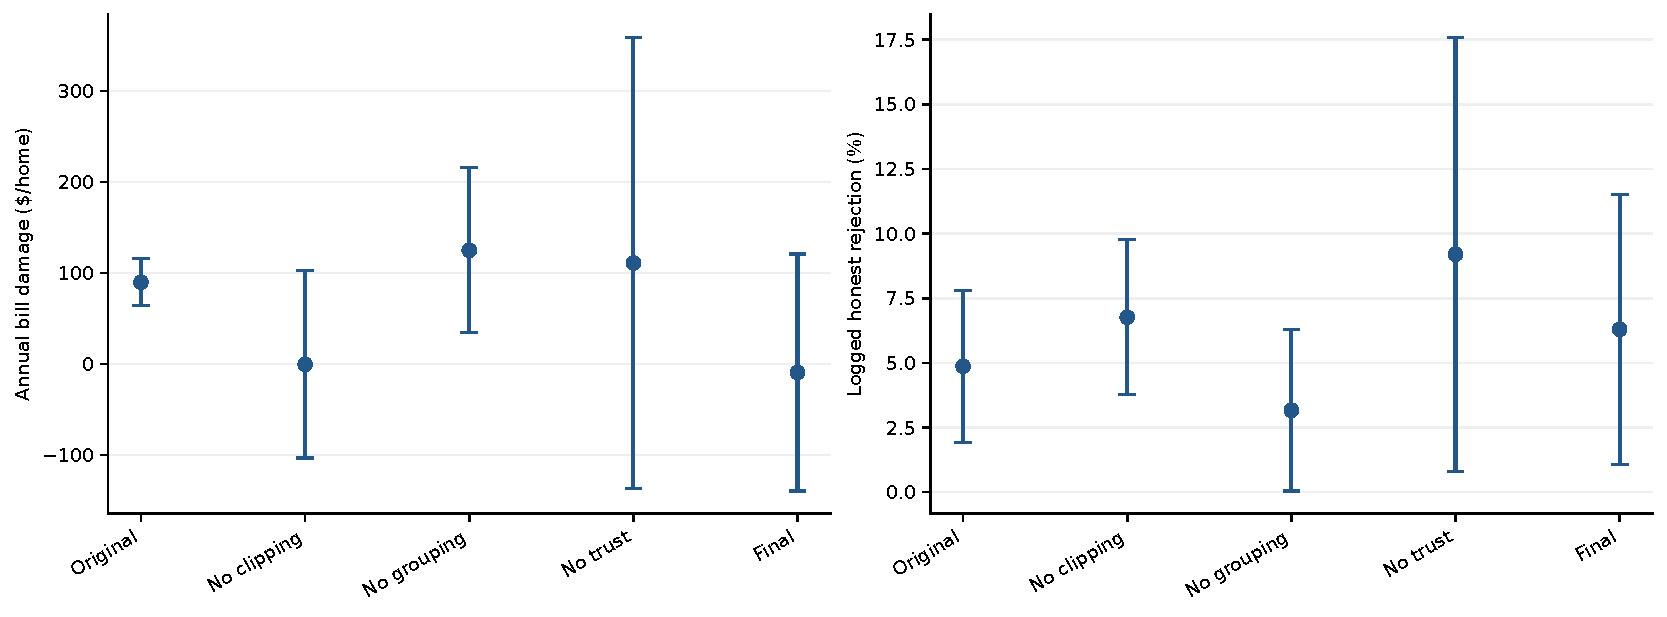
\includegraphics[width=\linewidth]{figures/ablation.pdf}
\caption{Original FedGrid ablations and final variant under Normalized attack, seeds 0--2. Error bars are unadjusted 95\% Student-$t$ intervals. Rejection refers to the logged admission mask. The final variant is a combined revision, not a single-factor ablation.}
\label{fig:ablation}
\end{figure}

\subsection{Communication faults, feeder size and voltage stress}
Table~\ref{tab:sensitivity} pairs each scenario with its same-method no-attack reference. Final FedGrid's Normalized damage is approximately $-\$18$ under the specified message faults, \$37 on feeder O and $-\$12$ at 1.02\,pu. Each is a single-seed sensitivity observation. Negative differences do not establish a benefit from faults or attacks. The large trimmed-mean damage under message faults is also consistent with a possible interaction between received-population size and share-dependent trimming, which the present cases do not isolate.
\begin{table}[htbp]
\centering\small
\caption{Normalized-attack damage under message faults, feeder O and 1.02 pu supply, seed 0. A dash means unavailable, not zero. Damage is in dollars per household per year, using the same variant and method no-attack reference.}
\label{tab:sensitivity}
\resizebox{\linewidth}{!}{%
\begin{tabular}{llll}
\toprule
Method & Lost/delayed (\$/home/yr) & Feeder O (\$/home/yr) & 1.02 pu (\$/home/yr) \\
\midrule
FedAvg & 529.2 [1] & 515.5 [1] & 614.6 [1] \\
Median & 261.9 [1] & -- & -- \\
Trimmed mean & 1224.0 [1] & -- & -- \\
Krum & -29.4 [1] & -- & -- \\
FLTrust & -37.0 [1] & 12.3 [1] & 32.4 [1] \\
FLAME & 2.3 [1] & 88.4 [1] & 25.0 [1] \\
TAFDRL-style & 10.5 [1] & -- & -- \\
TAFDRL-style tuned & 38.7 [1] & -- & -- \\
FedGrid original & 59.9 [1] & 137.9 [1] & -- \\
FedGrid final & -18.3 [1] & 36.7 [1] & -11.6 [1] \\
\bottomrule
\end{tabular}}
\end{table}

\begin{figure}[htbp]
\centering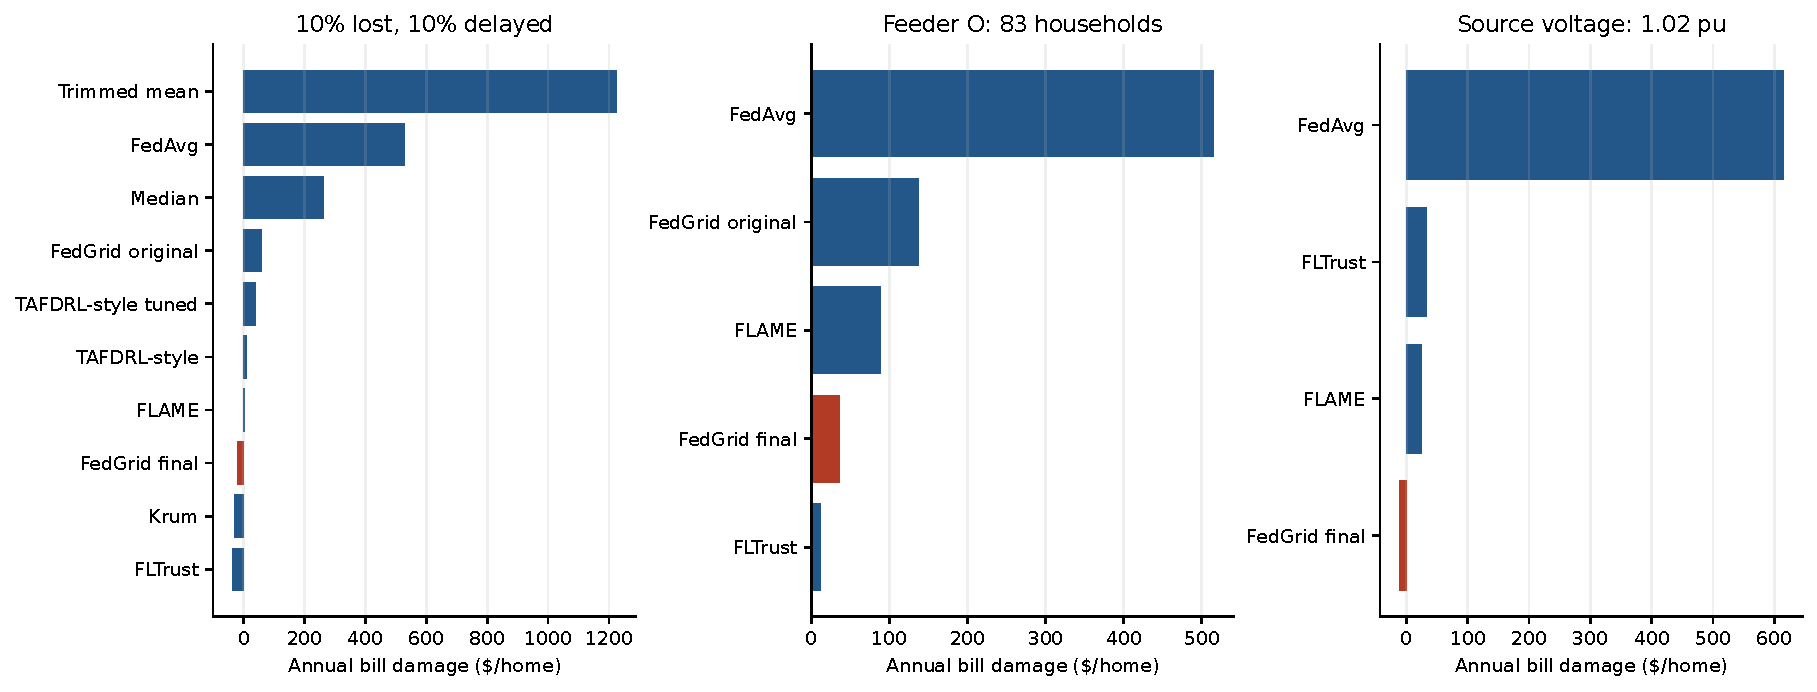
\includegraphics[width=\linewidth]{figures/sensitivity.pdf}
\caption{Normalized-attack damage in three sensitivity cases, seed 0. All-home annual bill differences use matched scenario references. Panels have different horizontal scales. Missing method--scenario combinations are not imputed.}
\label{fig:sensitivity}
\end{figure}

\subsection{Validation trajectories}
The trajectories show the mean and observed minimum--maximum range over seeds 0--2. They track validation-week cost plus the curtailment penalty, not annual evaluation bills. Reward-poisoned policies are assessed with ordinary observations after learning from reversed rewards. These are development diagnostics from the existing runs, not independent validation.
\begin{figure}[htbp]
\centering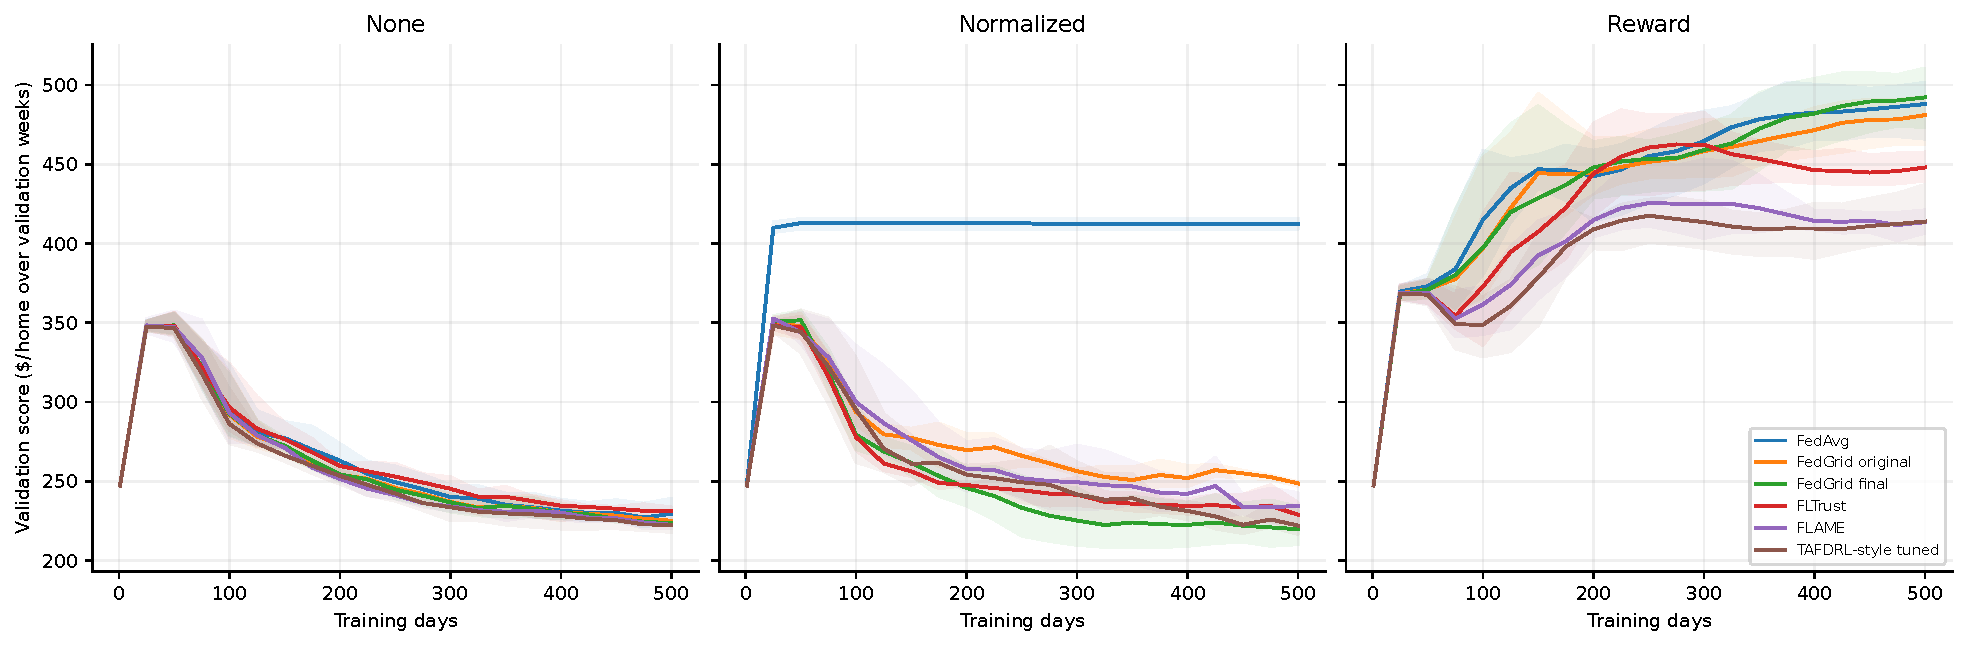
\includegraphics[width=\linewidth]{figures/training_curves.pdf}
\caption{Validation trajectories under no attack, Normalized attack and reward poisoning. Lines are three-seed means and shading is the observed seed range, not a confidence interval. Each panel shows validation objective values over training days.}
\label{fig:training}
\end{figure}

\subsection{Computational measurements}
The benchmark instantiates one household's actor and critics, containing 54,916 network values including local output layers. Table~\ref{tab:device} gives three repeated single-core trials on one Intel i7-10610U laptop; Linux peak-memory values are expressed in MiB. Shared-layer payload figures exclude local layers, optimiser state, target networks, protocol overhead and the reference learner. Server aggregation, transfers and the target embedded device would require separate deployment measurements.
\begin{table}[htbp]
\centering\small
\caption{Archived single-core laptop measurements (Intel i7-10610U). Three repeated timing trials on one device; these are not three independent hardware platforms.}
\label{tab:device}
\resizebox{\linewidth}{!}{%
\begin{tabular}{llll}
\toprule
Trial & Decision (ms) & Gradient step (ms) & Peak process memory (MiB) \\
\midrule
1 & 0.06 & 4.4 & 353 \\
2 & 0.04 & 4.1 & 356 \\
3 & 0.05 & 4.2 & 356 \\
\bottomrule
\end{tabular}}
\end{table}


\subsection{Computational reproducibility}
The accompanying artifacts contain per-seed outcomes, plotted values, analysis scripts and SHA-256 manifests. Statistical exports retain seed pairing and raw and adjusted p-values. Imputation records retain recipient and donor timestamps, their partitions and the denominators used for overlap fractions. Together, these records support reproduction of the analysis of existing experiments. Public archival identifiers and access terms have not been assigned.

\subsection{Audit of imputation donor overlap}
The donor audit reads raw ACT profiles and reconstructs the first observed value selected for each missing half hour by the fixed nearest-day rule. Reconstructed values are checked against the processed load and solar files at their stored precision. The audit uses the seed-zero evaluation street and its disjoint reference households. A profile cell denotes one household's load or solar value at one half hour; its denominator is distinct from a trajectory count or a household bill.

In the 36-home evaluation street, 2,004 training cells use donors from another partition, representing 0.259\% of training load-and-solar cells. Of these, 1,540 use evaluation-week donors. The reference street also contains 1,540 training cells with evaluation-week donors. The copied fraction alone does not bound its effect on policy selection or annual bills. A controlled rerun with partition-isolated preprocessing is needed to estimate that effect; this audit quantifies the overlap without correcting the reported experiments.
\begin{table}[htbp]
\centering\small
\caption{Read-only ACT imputation donor audit for the 36-home evaluation and reference streets. Counts pool load and solar half-hour cells. Cross-partition percentages use all profile cells in the recipient partition, not only filled cells. Copied evaluation data are a qualification of the existing evidence; no policy rerun is implied.}
\label{tab:imputation_audit}
\resizebox{\linewidth}{!}{%
\begin{tabular}{llrrrr}
\toprule
Street & Recipient partition & Filled cells & Cross-partition cells & Cross-partition (\%) & Donors from test \\
\midrule
Evaluation & train & 12,180 & 2,004 & 0.259 & 1,540 \\
Evaluation & validation & 2,980 & 388 & 0.229 & 0 \\
Evaluation & test & 3,168 & 396 & 0.126 & 2,772 \\
Reference & train & 12,748 & 2,000 & 0.258 & 1,540 \\
Reference & validation & 1,936 & 292 & 0.172 & 0 \\
Reference & test & 3,748 & 480 & 0.153 & 3,268 \\
\bottomrule
\end{tabular}}
\end{table}


\subsection{Exact paired statistical audit}
Two-sided exact Wilcoxon signed-rank tests compare five-seed Ausgrid damage. The robust-comparator family contains final FedGrid against FLTrust, FLAME and tuned TAFDRL-style across six attacks (18 tests). The revision family contains final against original FedGrid across the same six attacks. Holm adjustment is applied separately within each family. These are exploratory tests on already observed data, not a prospectively registered analysis.

All comparisons have nonzero differences and no tied absolute ranks. For five such pairs, the smallest attainable two-sided exact p-value is $2/2^5=0.0625$; a value below 0.05 is therefore unattainable even before adjustment. The Normalized final-minus-original comparison has exact p-value 0.0625 and six-test adjusted p-value 0.375. A descriptive Student-$t$ interval may exclude zero because the interval and rank test use different assumptions and formulations. Both results are reported with their scope, and all pair differences and p-values are exported as CSV.
\begin{table}[htbp]
\centering\small
\caption{Exploratory two-sided exact paired Wilcoxon tests on five Ausgrid seeds. Differences are final FedGrid minus the comparator. Holm adjustment uses 18 tests for robust comparators and six for the original-method revision; no adjusted test rejects at 0.05.}
\label{tab:exact_statistics}
\begin{tabular}{llrrr}
\toprule
Comparator & Attack & Mean difference (\$/yr) & Exact $p$ & Holm $p$ \\
\midrule
FLTrust & Flip & 68.1 & 0.0625 & 1.000 \\
FLTrust & Scale & -12.9 & 0.0625 & 1.000 \\
FLTrust & Noise & 33.0 & 0.1250 & 1.000 \\
FLTrust & Normalized & -11.8 & 0.8125 & 1.000 \\
FLTrust & Meter & 5.9 & 1.0000 & 1.000 \\
FLTrust & Reward & 42.8 & 0.0625 & 1.000 \\
FLAME & Flip & 14.0 & 0.1875 & 1.000 \\
FLAME & Scale & -19.5 & 0.3125 & 1.000 \\
FLAME & Noise & 17.3 & 0.3125 & 1.000 \\
FLAME & Normalized & -31.8 & 0.3125 & 1.000 \\
FLAME & Meter & 15.3 & 0.4375 & 1.000 \\
FLAME & Reward & 64.7 & 0.0625 & 1.000 \\
TAFDRL-style tuned & Flip & 29.7 & 0.3125 & 1.000 \\
TAFDRL-style tuned & Scale & -29.6 & 0.1250 & 1.000 \\
TAFDRL-style tuned & Noise & 22.6 & 0.0625 & 1.000 \\
TAFDRL-style tuned & Normalized & -27.7 & 0.6250 & 1.000 \\
TAFDRL-style tuned & Meter & 18.9 & 0.6250 & 1.000 \\
TAFDRL-style tuned & Reward & 42.4 & 0.1250 & 1.000 \\
FedGrid original & Flip & -10.4 & 0.3125 & 1.000 \\
FedGrid original & Scale & -5.3 & 0.6250 & 1.000 \\
FedGrid original & Noise & -28.4 & 0.0625 & 0.375 \\
FedGrid original & Normalized & -76.8 & 0.0625 & 0.375 \\
FedGrid original & Meter & 13.6 & 0.4375 & 1.000 \\
FedGrid original & Reward & 14.6 & 0.4375 & 1.000 \\
\bottomrule
\end{tabular}
\end{table}

